\documentclass{article}

% packages
  % basic stuff for rendering math
  \usepackage[letterpaper, top=1in, bottom=1in, left=1in, right=1in]{geometry}
  \usepackage[utf8]{inputenc}
  \usepackage[english]{babel}
  \usepackage{amsmath} 
  \usepackage{amssymb}
  % \usepackage{amsthm}

  % extra math symbols and utilities
  \usepackage{mathtools}        % for extra stuff like \coloneqq
  \usepackage{mathrsfs}         % for extra stuff like \mathsrc{}
  \usepackage{centernot}        % for the centernot arrow 
  \usepackage{bm}               % for better boldsymbol/mathbf 
  \usepackage{enumitem}         % better control over enumerate, itemize
  \usepackage{hyperref}         % for hypertext linking
  \usepackage{fancyvrb}          % for better verbatim environments
  \usepackage{newverbs}         % for texttt{}
  \usepackage{xcolor}           % for colored text 
  \usepackage{listings}         % to include code
  \usepackage{lstautogobble}    % helper package for code
  \usepackage{parcolumns}       % for side by side columns for two column code
  

  % page layout
  \usepackage{fancyhdr}         % for headers and footers 
  \usepackage{lastpage}         % to include last page number in footer 
  \usepackage{parskip}          % for no indentation and space between paragraphs    
  \usepackage[T1]{fontenc}      % to include \textbackslash
  \usepackage{footnote}
  \usepackage{etoolbox}

  % for custom environments
  \usepackage{tcolorbox}        % for better colored boxes in custom environments
  \tcbuselibrary{breakable}     % to allow tcolorboxes to break across pages

  % figures
  \usepackage{pgfplots}
  \pgfplotsset{compat=1.18}
  \usepackage{float}            % for [H] figure placement
  \usepackage{tikz}
  \usepackage{tikz-cd}
  \usepackage{circuitikz}
  \usetikzlibrary{arrows}
  \usetikzlibrary{positioning}
  \usetikzlibrary{calc}
  \usepackage{graphicx}
  \usepackage{caption} 
  \usepackage{subcaption}
  \captionsetup{font=small}

  % for tabular stuff 
  \usepackage{dcolumn}

  \usepackage[nottoc]{tocbibind}
  \pdfsuppresswarningpagegroup=1
  \hfuzz=5.002pt                % ignore overfull hbox badness warnings below this limit

% New and replaced operators
  \DeclareMathOperator{\Tr}{Tr}
  \DeclareMathOperator{\Sym}{Sym}
  \DeclareMathOperator{\Span}{span}
  \DeclareMathOperator{\std}{std}
  \DeclareMathOperator{\Cov}{Cov}
  \DeclareMathOperator{\Var}{Var}
  \DeclareMathOperator{\Corr}{Corr}
  \DeclareMathOperator{\pos}{pos}
  \DeclareMathOperator*{\argmin}{\arg\!\min}
  \DeclareMathOperator*{\argmax}{\arg\!\max}
  \newcommand{\ket}[1]{\ensuremath{\left|#1\right\rangle}}
  \newcommand{\bra}[1]{\ensuremath{\left\langle#1\right|}}
  \newcommand{\braket}[2]{\langle #1 | #2 \rangle}
  \newcommand{\qed}{\hfill$\blacksquare$}     % I like QED squares to be black

% Custom Environments
  \newtcolorbox[auto counter, number within=section]{question}[1][]
  {
    colframe = orange!25,
    colback  = orange!10,
    coltitle = orange!20!black,  
    breakable, 
    title = \textbf{Question \thetcbcounter ~(#1)}
  }

  \newtcolorbox[auto counter, number within=section]{exercise}[1][]
  {
    colframe = teal!25,
    colback  = teal!10,
    coltitle = teal!20!black,  
    breakable, 
    title = \textbf{Exercise \thetcbcounter ~(#1)}
  }
  \newtcolorbox[auto counter, number within=section]{solution}[1][]
  {
    colframe = violet!25,
    colback  = violet!10,
    coltitle = violet!20!black,  
    breakable, 
    title = \textbf{Solution \thetcbcounter}
  }
  \newtcolorbox[auto counter, number within=section]{lemma}[1][]
  {
    colframe = red!25,
    colback  = red!10,
    coltitle = red!20!black,  
    breakable, 
    title = \textbf{Lemma \thetcbcounter ~(#1)}
  }
  \newtcolorbox[auto counter, number within=section]{theorem}[1][]
  {
    colframe = red!25,
    colback  = red!10,
    coltitle = red!20!black,  
    breakable, 
    title = \textbf{Theorem \thetcbcounter ~(#1)}
  } 
  \newtcolorbox[auto counter, number within=section]{proposition}[1][]
  {
    colframe = red!25,
    colback  = red!10,
    coltitle = red!20!black,  
    breakable, 
    title = \textbf{Proposition \thetcbcounter ~(#1)}
  } 
  \newtcolorbox[auto counter, number within=section]{corollary}[1][]
  {
    colframe = red!25,
    colback  = red!10,
    coltitle = red!20!black,  
    breakable, 
    title = \textbf{Corollary \thetcbcounter ~(#1)}
  } 
  \newtcolorbox[auto counter, number within=section]{proof}[1][]
  {
    colframe = orange!25,
    colback  = orange!10,
    coltitle = orange!20!black,  
    breakable, 
    title = \textbf{Proof. }
  } 
  \newtcolorbox[auto counter, number within=section]{definition}[1][]
  {
    colframe = yellow!25,
    colback  = yellow!10,
    coltitle = yellow!20!black,  
    breakable, 
    title = \textbf{Definition \thetcbcounter ~(#1)}
  } 
  \newtcolorbox[auto counter, number within=section]{example}[1][]
  {
    colframe = blue!25,
    colback  = blue!10,
    coltitle = blue!20!black,  
    breakable, 
    title = \textbf{Example \thetcbcounter ~(#1)}
  } 
  \newtcolorbox[auto counter, number within=section]{code}[1][]
  {
    colframe = green!25,
    colback  = green!10,
    coltitle = green!20!black,  
    breakable, 
    title = \textbf{Code \thetcbcounter ~(#1)}
  } 

  \BeforeBeginEnvironment{example}{\savenotes}
  \AfterEndEnvironment{example}{\spewnotes}
  \BeforeBeginEnvironment{lemma}{\savenotes}
  \AfterEndEnvironment{lemma}{\spewnotes}
  \BeforeBeginEnvironment{theorem}{\savenotes}
  \AfterEndEnvironment{theorem}{\spewnotes}
  \BeforeBeginEnvironment{corollary}{\savenotes}
  \AfterEndEnvironment{corollary}{\spewnotes}
  \BeforeBeginEnvironment{proposition}{\savenotes}
  \AfterEndEnvironment{proposition}{\spewnotes}
  \BeforeBeginEnvironment{definition}{\savenotes}
  \AfterEndEnvironment{definition}{\spewnotes}
  \BeforeBeginEnvironment{exercise}{\savenotes}
  \AfterEndEnvironment{exercise}{\spewnotes}
  \BeforeBeginEnvironment{proof}{\savenotes}
  \AfterEndEnvironment{proof}{\spewnotes}
  \BeforeBeginEnvironment{solution}{\savenotes}
  \AfterEndEnvironment{solution}{\spewnotes}
  \BeforeBeginEnvironment{question}{\savenotes}
  \AfterEndEnvironment{question}{\spewnotes}
  \BeforeBeginEnvironment{code}{\savenotes}
  \AfterEndEnvironment{code}{\spewnotes}

  \definecolor{dkgreen}{rgb}{0,0.6,0}
  \definecolor{gray}{rgb}{0.5,0.5,0.5}
  \definecolor{mauve}{rgb}{0.58,0,0.82}
  \definecolor{lightgray}{gray}{0.93}

  % default options for listings (for code)
  \lstset{
    autogobble,
    frame=ltbr,
    language=C,                           % the language of the code
    aboveskip=3mm,
    belowskip=3mm,
    showstringspaces=false,
    columns=fullflexible,
    keepspaces=true,
    basicstyle={\small\ttfamily},
    numbers=left,
    firstnumber=1,                        % start line number at 1
    numberstyle=\tiny\color{gray},
    keywordstyle=\color{blue},
    commentstyle=\color{dkgreen},
    stringstyle=\color{mauve},
    backgroundcolor=\color{lightgray}, 
    breaklines=true,                      % break lines
    breakatwhitespace=true,
    tabsize=3, 
    xleftmargin=2em, 
    framexleftmargin=1.5em, 
    stepnumber=1
  }

% Page style
  \pagestyle{fancy}
  \fancyhead[L]{Frequentist Statistics}
  \fancyhead[C]{Muchang Bahng}
  \fancyhead[R]{December 2022} 
  \fancyfoot[C]{\thepage / \pageref{LastPage}}
  \renewcommand{\footrulewidth}{0.4pt}          % the footer line should be 0.4pt wide
  \renewcommand{\thispagestyle}[1]{}  % needed to include headers in title page

\begin{document}

\title{Frequentist Statistics}
\author{Muchang Bahng}
\date{December 2022}

\maketitle
\tableofcontents
\pagebreak

  We assume the reader is familiar with measure-theoretic probability, and unlike in introductory probability, we throw away the convention that random variables are written with capital Latin letters (so $x$ can also denote a random variable, which is useful if samples are not fixed). Statistics and probability seem like the same topic, but there are very fundamental differences. In probability, we are given some distribution and must compute certain probabilities. In statistics, we are given the results (the data) and must infer what distribution it came from. 

\section{Foundations}

  \subsection{Sampling Distributions}

    \begin{definition}[Population, Parameters]
      When conducting a statistical study, there is a set of items or events which is of interest for some experiment. This can be modeled with some probability space $(\Omega, \mathcal{F}, \mathbb{P})$. Usually, we are interested in some numerical property of this population, and so we implicitly define a random variable $X: \Omega \longrightarrow \mathbb{R}$ that induces some distribution $X \sim P$, which we call the \textbf{population}. A statistical population can be a group of existing objects or a hypothetical and potentially infinite group of objects conceived as a generalization from experience. 

      With this, we can interpret the population $X \sim P$ as a random variable, and we often call this the \textbf{parent distribution}. We are often interested in its population \textbf{parameters}, which can be any measured quantity of a population that summarizes or describes an aspect of it. In generality, the parameter of population $X$ is denoted $\theta$, and it is a fixed value. The two most useful ones are: 
      \begin{enumerate}
        \item the population mean $\mu_X$ 
        \item the population variance $\sigma^2_X$ 
      \end{enumerate}
    \end{definition}

    \begin{example}[Populations]
      Here are some examples of populations: 
      \begin{enumerate}
        \item We let $\Omega$ be the discrete sample space of all hands in poker, and our random variable will assign a numerical ranking to each hand $0$ for no hand, $1$ for pairs, $2$ for two pairs, etc. 
        \item $\Omega$ is the sample space of all individuals in the U.S. and we can construct a random variable $X$ that assigns to each individual their height. Even though $\Omega$ is finite, we can interpret it as continuous, which leads to a continuous distribution $X \sim P$. 
      \end{enumerate}
    \end{example}

    In general, the population is the total set of all relevant things that we are interested in. The specific quantity of the actual population is called the \textbf{population parameter}, e.g. the true mean $\mu$ or the true variance $\sigma^2$ of $X$, usually denoted with $\theta$. But usually, these parameters are not known since the population is too big to experimentally measure, so we must try and estimate it with samples. This is the entire point of statistics; otherwise, we would already know everything we want to know. 

    \begin{definition}[Samples]
      From the population $X \sim P$ (which still has unknown distribution), we can take $n$ \textbf{samples} by considering iid $x_1, x_2, \ldots, x_n \sim P$. 
      \begin{enumerate}
        \item We should note that the samples $x_i$ are random variables themselves. Not fixing them yet and still considering them in generality as random objects allows us to do more theoretical calculations. 
        \item Once these samples have been realized (i.e. $\omega \in \Omega$ is realized, and all $x_i$'s are also realized), we can treat them as fixed values. 
      \end{enumerate}
      Sometimes, we may not assume independence, but for most cases we do. A common rule is that if the sample size $n$ is less than 10\% of the population size, then we can assume independence. 
    \end{definition}

    \begin{definition}[Empirical Distribution]
      Now given that we have these iid samples, we can construct the \textbf{empirical distribution} $\widehat{X} \sim \widehat{P}$, defined as the discrete distribution that assigns probability $1/n$ to each value $x_i$ for $i \in [n]$. In other words, we have 
      \begin{equation}
        \mathbb{P}(\widehat{X} = x) = \frac{1}{n} \text{ for } x \in \{x_1, \ldots, x_n\}
      \end{equation}
      We can write the CDF of the empirical distribution, called the \textbf{empirical distribution function}, as the sum of indicators
      \begin{equation}
        F_X (x) = \frac{1}{n} \sum_{i=1}^n \mathbb{I}_{[x_i, +\infty)} (x)
      \end{equation}
    \end{definition}

    As expected, we would expect the empirical distribution to converge to the actual distribution. 

    \begin{theorem}[Glivenko–Cantelli theorem]
      The empirical distribution of iid samples $x_1, \ldots, x_n \sim P_n$ converges almost surely to $X \sim P$ as $n \rightarrow \infty$. More specifically, given that the CDF of $X$ is $F$ and the CDF of $P_n$ is the step function $F_n$, we have 
      \begin{equation}
        ||F_n - F||_{\infty} = \sup_{x \in \mathbb{R}} |F_n (x) - F(x)| \rightarrow 0
      \end{equation}
      almost surely as $n \rightarrow \infty$. 
    \end{theorem}

    \begin{example}[Empirical Distribution of Standard Gaussian]
      We expect the empirical distribution of the standard Gaussian to converge. Indeed, numerical results show that for 10 and 100 samples, the empirical CDF does converge to the true CDF. 

      \begin{center}
        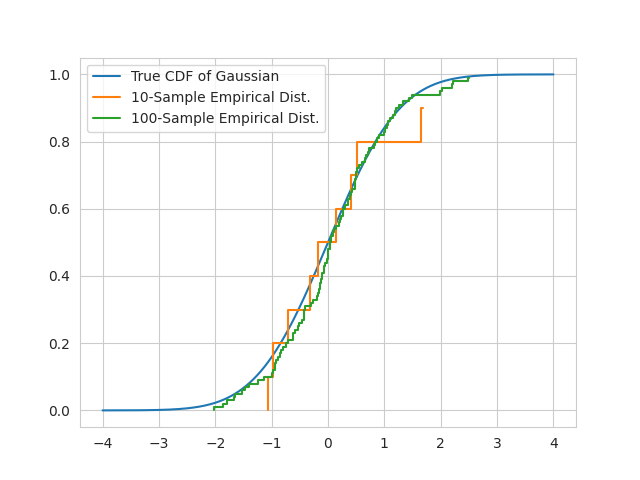
\includegraphics[scale=0.4]{img/empirical_distribution.png}
      \end{center}
    \end{example}

  \subsection{Concentration of Measure}

    Now let's move on to concentration inequalities, which say that the probability that a random variable is greater than something is bounded by something. These probability bounds are extremely useful in of themselves. It allows us to talk about convergence theory, which tells us what happens to a statistic, such as $\overline{X}$, as I get more and more data. The first inequality exploits the fact that the tails of a Gaussian RV decay very quickly, and a lot of concentration inequalities attempt to mimic this exponential bound but for non-Gaussian distributions. 

    \begin{theorem}[Gaussian Tail Inequality]
    Given $X \sim \mathcal{N}(0, 1)$, the inequality says that the probability of $X$ taking values past a certain $t$ decays exponentially. 
    \[\mathbb{P} \big( |X| > t \big) \leq \frac{2 e^{-t^2/2}}{t}\]
    If we have $x_1, \ldots, x_n \sim \mathcal{N}(0, 1)$, then 
    \[\mathbb{P} \big( |\overline{X}| > t \big) \leq \frac{2}{\sqrt{n} t} e^{-n t^2/2}\]
    We can assume that the coefficient is less than $1$ if $n$ is large. The above tells us that this bound exponentially decays with $t$ but also with the number of samples $n$. 
    \end{theorem}

    \begin{theorem}[Markov's Inequality]
    Given a nonnegative random variable $X > 0$, we have 
    \[\mathbb{P}(X > t) \leq \frac{\mathbb{E}[X]}{t}\]
    \end{theorem}
    \begin{proof}
    We have 
    \begin{align*}
        \mathbb{E}[X] & = \int_0^\infty x p_X (x)\,dx \\
        & \geq \int_t^\infty x p_X (x) \,dx \\
        & = t \int_t^\infty p_X (x) \,dx \\
        & = t \mathbb{P}(X > t)
    \end{align*}
    \end{proof}

    \begin{theorem}[Chebyshev's Inequality]
    Given a random variable $X$ with mean $\mu = \mathbb{E}[X]$, we have 
    \[\mathbb{P}\big( |x - \mu| > t\big) \leq \frac{\mathrm{Var}(X)}{t^2}\]
    \end{theorem}

    \begin{theorem}[Hoeffding's Inequality]
    Let $x_1, x_2, \ldots, x_n$ be independent (not necessarily identical) random variables s.t. $a_i \leq X_i \leq b_i$ almost surely. Consider the random variable $\overline{X} = \frac{1}{n} (x_1 + \ldots + x_n)$. Then, for all $t > 0$, 
    \[\mathbb{P}\big( \big| \overline{X} - \mathbb{E}[\overline{X}] \big| \geq t \big) \leq 2 \exp \bigg( -\frac{2 n^2 t^2}{\sum_{i=1}^n (b_i - a_i)^2} \bigg)\]
    \end{theorem}

    Now in addition to bounding probabilities, we would like to bound expectations. 

    \begin{theorem}[Cauchy-Schwartz]
    Given random variables $X, Y$, it is often hard to compute the expectation of $X Y$ since it is hard to compute the distribution of it (sums are easy). But we can bound it as 
    \[|\mathbb{E}[XY]| \leq \mathbb{E}[ |XY| ] \leq \sqrt{\mathbb{E}[X] \, \mathbb{E}[Y]}\]
    \end{theorem}

    \begin{theorem}[Jensen's Inequality]
    Given $g$ a convex function and $X$ a random variable, we have 
    \[\mathbb{E}[ g(X)] \geq g (\mathbb{E}[X])\]
    \end{theorem}

    \subsection{Kullback Leibler Divergence}

    Now a popular metric between PMFs/PDFs is the KL divergence. 

    \begin{definition}[Kullback-Leibler Divergence]
    Given random variable $X$ and $Y$, 
    \begin{enumerate}
        \item If they are discrete with PMFs $P$ and $Q$, the KL-divergence is defined 
        \[D_{KL} (P \mid\mid Q) \coloneqq \sum_{x} P(x) \, \log \bigg(\frac{P(x)}{Q(x)} \bigg) = \mathbb{E} \bigg[ \log \frac{P(x)}{Q(x)} \bigg] \]
        where we can interpret the expectation as $X \sim p$. 
        \item If they are continuous with PDFs $p$ and $q$, the KL-divergence is defined 
        \[D_{KL} (p \mid\mid q) \coloneqq \int p(x) \, \log \bigg( \frac{p(x)}{q(x)} \bigg)\,dx = \mathbb{E} \bigg[ \log \frac{P(x)}{Q(x)} \bigg] \]
        where we can interpret the expectation as $X \sim p$. 
    \end{enumerate}
    \end{definition}

    We should prove that this is indeed a metric. 
    \begin{enumerate}
        \item The fact that $D_{KL} (p \mid p) = 0$ is obvious. 
        \item To prove that $D_{KL} (p \mid q) \geq 0$, we use Jensen's inequality
        \[-D_{KL} (p \mid q) = \mathbb{E} \log \frac{q(X)}{p(X)} \leq \log \mathbb{E} \frac{q(X)}{p(X)} = \log \int \frac{q(x)}{p(x)} \, p(x) \, dx = \log(1) = 0\]
        It is a common trick to switch the log and the expectation using Jensen's. 
    \end{enumerate}

    \subsection{Bounding Maximum of Random Variables}

    Given that we have $n$ samples $x_1, \ldots, x_n \sim P$, it is conventional to index them with open brackets to denote order 
    \[X_{(1)} \leq X_{(2)} \leq \ldots \leq X_{(n)}\]
    Our goal is now to find the distribution of $X_{(n)} = \max_i X_i$. If we know the distribution of $P$, $\mathbb{P}(X_{(n)} \leq x)$ is just the probability that all the $X_i$'s are less than $x$, and by independence we can product out the CDFs, differentiate to get the PDF, and compute. So it's not too hard to do this theoretically, but in practice this is hard to do since we don't exactly know $P$. 

    So if you didn't know the $X_i$'s, the best you can assume is that 
    \[\mathbb{E} \max\{x_1, \ldots, x_n\}\]
    is going to grow like $n$. But if we can bound the MGF with $\mathbb{E} e^{t X} \leq e^{t^2 \sigma^2}{2}$, then we can show that $\mathbb{E} \max X_i$ doesn't grow like $n$, but rather like $\log{n}$. 
    \[\mathbb{E} \max{X_i} \leq \sigma \sqrt{2 \log{n}}\]

    \subsection{Big-O, Little-O Notation}

    Going back to calculus, if we have a function $f: X \longrightarrow \mathbb{R}$, we can say that 
    \begin{enumerate}
        \item $f(x) = O(g(x))$ if $f$ is of the same order as $g$. That is, they grow at the same rate 
        \[\frac{f(x)}{g(x)} \rightarrow c \text{ as } x \rightarrow \infty\]
        for some constant $c$. 
        \item $f(x) = o(g(x))$ if $f$ is negligible w.r.t. $g$. That is, $f$ is infinitesimal w.r.t. $g$. 
        \[\frac{f(x)}{g(x)} \rightarrow 0 \text{ as } x \rightarrow \infty\]
        for some constant $c$. 
    \end{enumerate}
    Now there is a probabilistic notation as well. The concept of boundedness translates to being able to capture most of the mass of the random variable within some interval, and infinitesimality translates to the probability mass concentrating around $0$. 

    \begin{definition}[$O_p, o_p$ Notation]
    Let $x_1, x_2, \ldots $ be a sequence of random variables. 
    \begin{enumerate}
        \item $x_n = o_p (1)$ if 
        \[\mathbb{P}(|Y_n| > \epsilon) \rightarrow 0 \text{ as } n \rightarrow \infty\]
        for all $\epsilon > 0$. This means that $x_n$ gets more and more concentrated around $0$. 

        \item $x_n = O_p(1)$ if for all $\epsilon > 0$, then there exists a $C$ s.t. 
        \[\mathbb{P}(|x_n| > C) \leq \epsilon\]
        for all large $n$. That is, we can always trap the majority of the probability mass of $x_n$ within the interval $[-C, C]$. This must hold for all $x_n$ with $n > N$, so the mass can't "escape" to infinity. We can think of it as the distribution is "settling down" and not shooting off to somewhere. 

        \item $x_n = o_p (a_n)$ means that 
        \[\frac{x_n}{a_n} = o_p (1)\]

        \item $x_n = O_p (a_n)$ means that 
        \[\frac{x_n}{a_n} = O_p(1)\]
    \end{enumerate}
    \end{definition}

    \begin{theorem}
    Given $Y_1, \ldots Y_n \sim \mathrm{Bernoulli}(p)$, let $\widehat{p} = \frac{1}{n} \sum Y_i$. Then 
    \[\widehat{p}_n - p = o_p (1)\]
    which is also written $\widehat{p}_n = p + o_p (1)$, which means that the random variable $\widehat{p}_n$ is some constant $p$ plus a random variable that is going to $0$. 
    \end{theorem}
    \begin{proof}
    By Hoeffding's inequality, 
    \[\mathbb{P}(| \widehat{p}_n - p | > \epsilon) \leq 2 e^{-2n \epsilon^2}\]
    which goes to $0$ as $n \rightarrow \infty$. 
    \end{proof}

    \begin{example}
    Given $Y_1, \ldots Y_n \sim \mathrm{Bernoulli}(p)$, let $\widehat{p} = \frac{1}{n} \sum Y_i$. Then, 
    \[\widehat{p} - p = O_p \Big( \frac{1}{\sqrt{n}} \Big)\]
    \end{example}

\section{Point Estimation}

    \begin{definition}[Sample Statistic, Estimators and Estimates]
      Now given a population $X$, we would like to use the $n$ iid samples $x_1, \ldots, x_n$ to estimate a parameter $\theta$ of interest with our own random variable/value $\widehat{\theta}_n$, called a \textbf{sample statistic}. We must note the dual nature of the sample statistic as a random variable and a value is similar to that of samples. 
      \begin{enumerate}
        \item The statistic $\widehat{\theta}_n$ is a random variable itself, referred to as the \textbf{estimator}. More specifically, it is a function $\widehat{\theta}_n: \mathbb{R}^n \longrightarrow \mathbb{R}$ of the $n$ samples, i.e. a transformation of random variables 
        \begin{equation}
          \widehat{\theta}_n = \widehat{\theta}_n (x_1, x_2, \ldots, x_n)
        \end{equation}
        This makes $\widehat{\theta}_n$ also a random variable, which attempts to estimate the true $\theta$, which is some unknown fixed value. Since $\widehat{\theta}_n$ is a random variable, it has its own distribution, called the \textbf{sampling distribution} of $\widehat{\theta}_n$. 
        
        \item Once these samples $x_i$ have been realized, the estimator realizes and the value realized is now called the \textbf{estimate}. 
      \end{enumerate}
      This sampling distribution is a distribution of the statistic $\widehat{\theta}_n$, and this forms a separate distribution with its own mean and variance. 
      \begin{enumerate}
        \item the mean of the sampling distribution is denoted $\mu_{\widehat{\theta}_n}$
        \item the standard deviation of the sampling distribution is denoted $\sigma^2_{\widehat{\theta}_n}$, also called the \textbf{standard error}. 
      \end{enumerate}
    \end{definition}

    We would want these estimators to have three properties: 
    \begin{enumerate}
      \item unbiasedness
      \item consistency 
      \item efficiency
    \end{enumerate}

    We would like the sampling distribution of our statistic to give us good estimate in two ways. $\widehat{\theta}_n$ should not be too far off from the actual parameter $\theta$ (bias is small), and $\widehat{\theta}_n$ should not fluctuate too widely (variance of $\widehat{\theta}_n$ should be small). 

    \begin{definition}[Bias, Variance of Estimator]
      Given an estimator $\widehat{\theta}$ of a sample $x_1, \ldots, x_n$ estimating population parameter $\theta$, the \textbf{sampling bias} refers to 
      \begin{equation}
        \mathrm{Bias}(\widehat{\theta}) = \big| \mathbb{E}[\widehat{\theta}] - \theta \big|
      \end{equation}
      and the \textbf{sampling variance} refers to 
      \begin{equation}
        \mathrm{Var}(\widehat{\theta}) = \mathbb{E} \big[ (\widehat{\theta} - \mathbb{E}[\widehat{\theta}])^2 \big]
      \end{equation}
    \end{definition}

    A good rule of thumb to remember is that statistics is about replacing expectations with averages. 
    \begin{equation}
      \mathbb{E} \mapsto \frac{1}{n} \sum_i
    \end{equation}
    This is really the fundamental quality of statistics. Then after that we can do some fancy things, like minimizing something or manipulating another, but every single time we see an expectation just replace it with an average. 

    \begin{definition}[Sample Mean]
      Given a population $X$ with $\mu = \mathbb{E}[X]$ and $\sigma^2 = \mathrm{Var}(X)$, our estimator for $\mu$ is simply the average of the $n$ samples $x_1, \ldots, x_n$, called the \textbf{sample mean} or the \textbf{sampling distribution of the sample mean}. 
      \begin{equation}
        \overline{x}_n = \widehat{\mu}_n = \frac{1}{n} (x_1 + \ldots + x_n)
      \end{equation}
      This gives us the sampling distribution of the sample means. The mean and standard deviation (i.e. standard error) of $\overline{x}_n$ is denoted $\mu_{\overline{x}_n}$ and $\sigma_{\overline{x}_n}$. 
      \begin{enumerate}
        \item The mean of $\overline{x}_n$ is $\mu$. 
        \begin{equation}
          \mu_{\overline{x}_n} = \mu
        \end{equation}
        because
        \begin{equation}
          \mathbb{E}[\overline{x}_n] = \mathbb{E} \bigg[ \frac{1}{n} \sum_{i=1}^n x_i \bigg] = \frac{1}{n} \sum_{i=1}^n \mathbb{E}[x_i] = \mathbb{E}[x] = \mu
        \end{equation}
        
        \item The variance of $\overline{x}_n$ is $\sigma^2 / n$, i.e. the standard error of $\overline{x}_n$ is $\sigma_{\overline{x}_n} = \sigma / \sqrt{n}$. 
        \begin{equation}
          \sigma_{\overline{x}_n} = \frac{\sigma}{\sqrt{n}}
        \end{equation}
        because 
        \begin{equation}
          \sigma^2_{\overline{x}_n} = \frac{1}{n^2} \sum_{i=1}^n \mathrm{Var}(x_i) = \frac{1}{n} \mathrm{Var}(x) = \frac{\sigma^2}{n}
        \end{equation}
         Practically, this tells us that when trying to estimate the value of a population mean, due to the factor of $1/\sqrt{n}$, reducing the error on the estimate by a factor of $2$ requires acquiring $4$ times as many observations in the sample. But realistically, the true standard deviation $\sigma$ is unknown, and so the standard error of the mean is usually estimated by replacing $\sigma$ with the sample standard deviation $S$ instead. 
        \begin{equation}
          \sigma_{\overline{x}_n} \approx \frac{S}{\sqrt{n}}
        \end{equation}

        \item By CLT, $\overline{x}_n$ converges to $\mathcal{N}(\mu, \sigma^2/n)$ in distribution as $n \rightarrow +\infty$ (but in practicality, we assume this for $n \geq 30$). The fact that its mean and variance is $\mu$ and $\sigma^2 /n$ isn't that impressive. What is really impressive is that no matter what the distribution of $x$ is, the sampling distribution of the mean will be Gaussian. 
      \end{enumerate}
    \end{definition}

    \begin{example}[Sample Means]
      Here are some figures of sample means. Note that with a uniform parent distribution, the sampling distribution of its mean looks like a Gaussian even without a large $n$. However, this is not necessarily true for different parent distributions, such as the exponential. 
      \begin{figure}[H]
        \centering
        \begin{subfigure}[b]{0.48\textwidth}
        \centering
          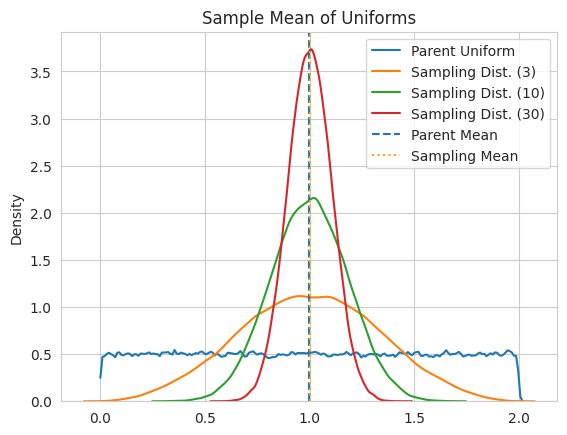
\includegraphics[width=\textwidth]{img/sample_mean_uniform.png}
          \caption{We plot the PDF of an $X \sim \mathrm{Uniform}[0, 2]$ random variable by taking 100k samples. We also take 100k samples from the sampling distribution of the mean $\overline{X}_{3}, \overline{X}_{10}, \overline{X}_{30}$. We can see that the standard deviation decreases by a factor of $\sqrt{n}$.}
          \label{fig:sample_mean_uniform}
        \end{subfigure}
        \hfill 
        \begin{subfigure}[b]{0.48\textwidth}
        \centering
          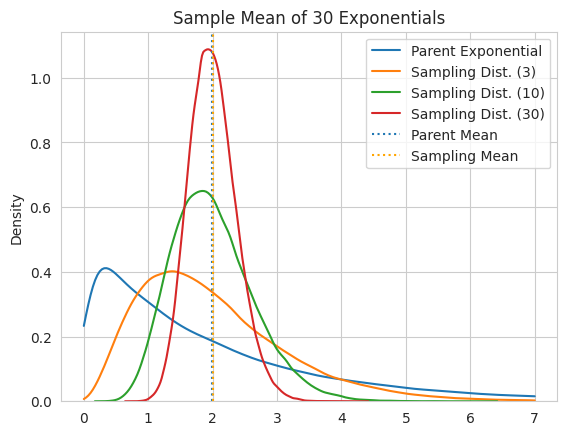
\includegraphics[width=\textwidth]{img/sample_mean_exp.png}
          \caption{We plot the PDF of an $X \sim \mathrm{Exponential}(1.5)$ random variable by taking 100k samples. We also take 100k samples from the sampling distribution of the mean $\overline{X}_{3}, \overline{X}_{10}, \overline{X}_{30}$. }
          \label{fig:sample_mean_exp}
        \end{subfigure}
        \caption{}
        \label{fig:sample_mean_examples}
      \end{figure}
    \end{example}

    If the parent distribution is normal, then we don't even need CLT to claim that the sampling distribution of the sample mean is normal, since sums of normals are normal. 

    Now the variance of the population is defined to be $\sigma^2 = \mathbb{E}[ (X - \mathbb{E}[X])^2 ]$, and by our rule of thumb, we can replace the expectations with sample means, by first setting $\mathbb{E}[X] = \widehat{\mu}$ and averaging out the values $(X - \widehat{\mu})^2$. 

    \begin{definition}[Sample Variance]
      Given a population $X$, our estimator for $\sigma^2 = \mathbb{E}[ (X - \mathbb{E}[X])^2 ]$ is simply the average of the squared distances of the $n$ samples $\{(x_i - \widehat{\mu})^2\}_{i=1}^n$. 
      \begin{equation}
        S^2_n = \widehat{\sigma}^2_n = \frac{1}{n} \sum_{i=1}^n ( x_i - \overline{x}_n)^2
      \end{equation}
      The mean and standard deviation of $S^2_n$ is denoted $\mu_{S^2_n}$ and $\sigma_{S^2_n}$. Note that there is a small difference that the sum for variance is divided by $n-1$ rather than $n$, since we want it to be unbiased, but we will correct this later. 
    \end{definition}

    While the CLT states that the sampling distribution of the sample mean will look approximately Gaussian, we do not have this luxury when looking at the sampling distribution of sample variance. 

    \begin{example}[Sample Variance]
      Take a look at the following sampling distributions of the sample variance. There does not seem to be strong signs of convergence to a Gaussian. Their means do not align either. 
      \begin{figure}[H]
        \centering
        \begin{subfigure}[b]{0.48\textwidth}
        \centering
          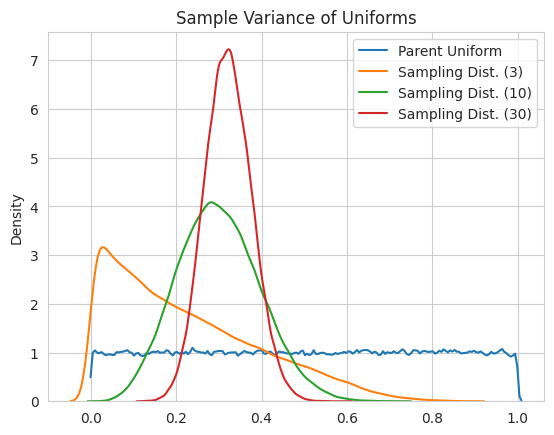
\includegraphics[width=\textwidth]{img/sample_variance_uniform.png}
          \caption{}
          \label{fig:sample_variance_uniform}
        \end{subfigure}
        \hfill 
        \begin{subfigure}[b]{0.48\textwidth}
        \centering
          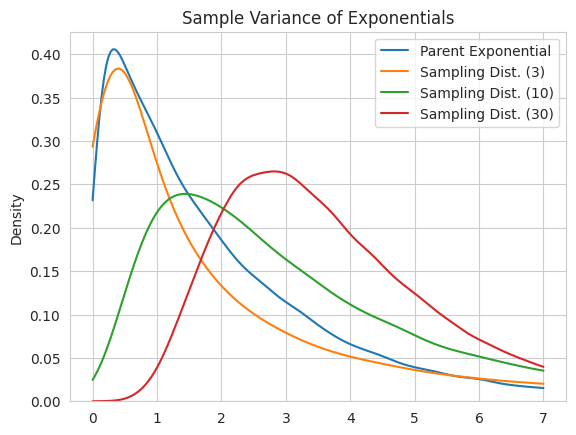
\includegraphics[width=\textwidth]{img/sample_variance_exp.png}
          \caption{}
          \label{fig:sample_variance_exp}
        \end{subfigure}
        \caption{}
        \label{fig:sample_variance_examples}
      \end{figure}
    \end{example}

  \subsection{Sampling from Gaussians}

    Now if we assume that the parent distribution is Gaussian, then we can conclude some extra things and more kinds of distributions arise. Let $x_1, \ldots, x_n \sim \mathcal{N}(\mu, \sigma^2)$, with $\overline{x}_n$ the sample mean and $S^2_n$ the sample variance. Say that we want to find the distribution of $\overline{x}_n$. 
    \begin{enumerate}
      \item In the unrealistic case where we know the true $\sigma^2$, we don't even need to consider the sample variance. From the basic property of Gaussians, we know that $\overline{x}_n \sim \mathcal{N}(\mu, \sigma^2/n)$, or after standardizing, 
      \begin{equation}
        \frac{\overline{x}_n - \mu}{\sigma/\sqrt{n}} \sim \mathcal{N}(0, 1)
      \end{equation}
      \item In the realistic case where we don't know the true $\sigma^2$, we should replace it with our sample variance $S^2$, and it turns out that because of this extra uncertainty in the variance, our sampling distribution follows the student-t distribution, which can be interpreted as a mixture of Gaussians with differing variances. 
      \begin{equation}
        \frac{\overline{x}_n - \mu}{S/\sqrt{n}} \sim \mathrm{StudentT}(n-1)
      \end{equation}
    \end{enumerate}
    Now if we are interested in finding the distribution of $S^2_n$: 
    \begin{enumerate}
      \item In the unrealistic case where the know the true $\mu$, we don't need to consider the sampling distribution of $\overline{x}_n$. We have 
      \begin{equation}
        S^2_n = \frac{1}{n} \sum_{i=1}^n (x_i - \mu)^2 \sim \mathrm{Gamma}\Big( \frac{n}{2}, \frac{n}{2 \sigma^2} \Big)
      \end{equation}
      \item In the realistic case where we don't know $\mu$, we have 
      \begin{equation}
        \frac{n-1}{\sigma^2} S^2_n = \frac{1}{\sigma^2} \sum_{i=1}^n (x_i - \overline{x}_n )^2 \sim \chi^2 (n-1)
      \end{equation}
    \end{enumerate}

  \subsection{Method of moments}

  \subsection{Maximum likelihood estimation}

  \subsection{Least squares estimation}

\section{Confidence Intervals}

    Recall that the central limit theorem says that given a sequence of iid random variables $x_1, \ldots, x_n$ coming from a random variable with true mean $\mu$ and variance $\sigma^2$, the sample mean is similar to a $\mathcal{N}(\mu, \sigma^2 / n)$ random variable. That is, the sample mean converges in distribution 
    \begin{equation}
      \overline{X}_n \xrightarrow{dist} \mathcal{N} \Big( \mu, \frac{\sigma^2}{n} \Big)
    \end{equation}
    as $n \rightarrow \infty$. Another way to state it is that the normalized sample mean is similar to a standard Gaussian. 
    \begin{equation}
      \frac{\overline{x}_n - \mu}{\sigma_{\overline{x}_n}} = \frac{\overline{x}_n - \mu}{\sigma / \sqrt{n}} \xrightarrow{dist} \mathcal{N}(0, 1)
    \end{equation}
    So, given that we have enough samples, I will perfectly understand its fluctuations. Now let's introduce some definitions that will allow us to unify some ideas into simpler notation: the realized value $x$, the number of standard deviations it is away from the mean, and the probability that it takes that value (or more extreme). 

    \begin{definition}[z-score]
      Given a $\mathcal{N}(\mu, \sigma^2)$ distribution, the \textbf{z-score} of a number $x \in \mathbb{R}$ is defined to be the number of standard deviations away from the mean. 
      \begin{equation}
        z = \frac{x - \mu}{\sigma}
      \end{equation}
    \end{definition}

    \begin{definition}[Percentile]
      Given $X \sim \mathcal{N}(0, 1)$ and significance level $\alpha \in [0, 1]$, let us define $q_{\alpha} \in \mathbb{R}$ as the point where 
      \begin{equation}
        \mathbb{P}(X \geq q_{\alpha}) = \alpha
      \end{equation}
      i.e. the $100\alpha$th percentile of the standard normal. Note that given $X \sim \mathcal{N}(0, 1)$, we have 
      \begin{equation}
        \mathbb{P} (|X| > q_{\alpha/2}) = \alpha
      \end{equation}
    \end{definition}

    Now given $x_1, \ldots, x_n$ from a population $X$ with mean $\mu$ and standard deviation $\sigma$, let $\overline{x}_n$ be the sampling distribution of the mean. By virtue of the central limit theorem, we can write
    \begin{equation}
      \mathbb{P} \bigg( \bigg| \frac{\overline{X}_n - \mu}{\sigma / \sqrt{n}} \bigg| \geq q_{\alpha/2} \bigg) \approx \alpha \iff \mathbb{P} \bigg( \bigg| \frac{\overline{X}_n - \mu}{\sigma \sqrt{n}} \bigg| \leq q_{\alpha/2} \bigg) \approx 1 - \alpha
    \end{equation}
    which implies that with probability $1 - \alpha$, we have 
    \begin{equation}
      \overline{X}_n \in \bigg[ \mu - q_{\alpha/2} \frac{\sigma}{\sqrt{n}}, \mu + q_{\alpha/2} 
      \frac{\sigma}{\sqrt{n}} \bigg] \iff \mu \in \bigg[ \overline{X}_n - q_{\alpha/2} \frac{\sigma}{\sqrt{n}}, \overline{X}_n + q_{\alpha/2} \frac{\sigma}{\sqrt{n}} \bigg]
    \end{equation}
    This is how we construct a confidence interval. In other words, as $n$ becomes large (ideally at least $30$), the probability that an interval around our sample mean contains the actual mean $\mu$ can be approximated by a Gaussian. But note that CI requires to know the actual standard deviation $\sigma$. There are three ways to deal with this: 
    \begin{enumerate}
      \item This may actually be known from the start, especially if we are working with calibrated devices with standard devices that have been experimentally verified.

      \item We can simply bound $\sigma$, depending on what kind of random variable we are working with. For example, given $X \sim \mathrm{Bernoulli}(p)$, its standard deviation is bounded by $\sigma = \sqrt{p (1 - p)} \leq \frac{1}{2}$, so we can create a confidence interval that is larger than any other confidence interval we can make if we had known the true $\sigma$. 
      \begin{equation}
        p \in \bigg[ \overline{X}_n - q_{\alpha/2} \, \frac{1}{2 \sqrt{n}}, \overline{X}_n + q_{\alpha/2} \,\frac{1}{2 \sqrt{n}} \bigg]
      \end{equation}

      \item We can approximate $\sigma$ with the sample standard deviation $S$, which turns out to be an unbiased estimator. 
    \end{enumerate}

    \begin{example}[Proportion of Right-Side Kissers]
      We have observed $80$ out of $124$ right-side kisses, resulting in a sample estimate of $\widehat{p} = 0.645$. Given that we want a confidence interval of $95\%$, we want an $\alpha = 0.05$, implying a the value $q_{\alpha/2} = q_{0.025} = 1.96$. So, with probability $0.95$, we have 
      \begin{equation}
        p \in \bigg[ 0.645 - \frac{1.96}{2 \sqrt{124}}, 0.645 + \frac{1.96}{2 \sqrt{124}} \bigg] = [ 0.56, 0.73 ]
      \end{equation}
      If we had, say $3$ observations, rather than $124$, we would have a $95\%$ confidence interval of $p \in [0.10, 1.23]$, which is terrible, but in this case even CLT is not valid. 
    \end{example}

    \begin{example}[Proportion of Voters]
      Given that we sample $n = 100$ people from a city's population to ask whether they support candidate A or B, we have $54$ people who support candidate $A$, so $\widehat{p} = 0.54$. Say that we want a 95\% confidence interval, which leads to $q_{\alpha /2} = q_{0.025} = 1.96$. So, with probability $0.95$, we have 
      \begin{equation}
        p \in \bigg[ 0.54 - 1.96\,\frac{\sigma}{\sqrt{100}}, 0.54 + 1.96\,\frac{\sigma}{\sqrt{100}} \bigg]
      \end{equation}
      and by substituting $\sigma$ for $S = \sqrt{0.54 (1 - 0.54)} \approx 0.5$, we get 
      \begin{equation}
        p \in \bigg[ 0.54 - 1.96\,\frac{0.284}{\sqrt{100}}, 0.54 + 1.96\,\frac{0.284}{\sqrt{100}} \bigg] = [0.44, 0.64]
      \end{equation}
    \end{example}

    An interpretation of confidence intervals is that if you keep on sampling $\overline{x}$ or $\widehat{p}$ and construct 95\% CIs, then 95\% of the time these intervals will contain the true mean $\mu$ or proportion $p$ (or more if we had bounded the CI with a bigger interval). 

    \begin{example}
      We survey 6250 teachers to ask whether they think computers are essential for teaching. 250 were randomly selected and 142 felt that they were essential. Let's construct a 99\% confidence interval for the proportion of teachers who felt that computers were essential. We would like to construct a CI for the true $\mu = p$, and we have $\overline{x} = 142/250 = 0.568$. 
      \begin{enumerate}
        \item 99\% confidence corresponds to $\alpha = 0.01$, which corresponds to a z-score of $q_{\alpha/2} = 2.576$. 
        \item The parent distribution is $\mathrm{Bernoulli}(p)$, with $\mu = p$ and $\sigma = \sqrt{p (1 - p)}$. The sampling distribution of $\overline{x}$ has $\mu_{\overline{x}} = p$ also and $\sigma_{\overline{x}} = \sigma / \sqrt{n}$. 
        \item We need to know the details of the sampling distribution, but we don't know $\sigma$, which is needed to calculate $\sigma_{\overline{x}}$. However, we can estimate it using the sample standard deviation $S = \sqrt{0.568 (1 - 0.568)} = 0.5$. 
        \item Our sampling distribution has standard deviation $\sigma_{\overline{x}} \approx S / \sqrt{n} = 0.5 / \sqrt{250} = 0.031$, and our z-score was $2.576$, so our 99\% confidence interval is $2.576$ standard deviations from our mean. That is, with probability $0.99$, 
        \begin{equation}
          p \in \big[ 0.568 - 2.576 \cdot 0.031, 0.568 + 2.576 \cdot 0.031 \big] = \big[ 0.488144, 0.647856 \big]
        \end{equation}
      \end{enumerate}
    \end{example}

  \subsection{CIs for means, proportions, and variances}

  \subsection{Bootstrap confidence intervals}

\section{Hypothesis Testing}

    A significance test is a method used to decide whether the data at hand sufficiently supports a particular hypothesis. The hypothesis to be tested is called the \textbf{alternative hypothesis}, denoted $H_1$ or $H_a$, and the status quo is called the \textbf{null hypothesis}, denoted $H_0$. Assuming that $H_0$ is true, we compute the likelihood of the data happening. If the sample is not too unlikely (past some significance level), we fail to reject $H_0$, and if there is strong evidence, we reject $H_0$. $H_0$ and $H_a$ can be devised in countless ways. 

    \begin{example}
      There are countless test statistics we can build, but here are some common examples, 
      \begin{enumerate}
        \item Proportion: Company A produces circuit boards, but 10\% of them are defective. Company B claims that they produce fewer defective circuit boards. 
        \begin{equation}
          H_0 : \, p = 0.10 \text{ versus } H_a : \, p < 0.10
        \end{equation}
        
        \item Means: It is known that the average height of boys in KIS is 176cm. Ben claims that the average height is lower than this. 
        \begin{equation}
          H_0 : \, \mu = 176 \text{ versus } H_a : \, \mu < 176
        \end{equation}
        
        \item Difference of Means: If $\mu_1$ and $\mu_2$ denote the true average breaking strengths of the same type of twine produced by two different companies. Jenny claims that the $\mu_1 - \mu_2 > 5$. 
        \begin{equation}
          H_0 : \, \mu_1 - \mu_2 = 0 \text{ versus } H_a : \, \mu_1 - \mu_2 > 5
        \end{equation}
      \end{enumerate}
    \end{example}

  \subsection{One Sample Z and T Tests}

    Let us have some population $X \sim P$ and a null hypothesis that claims $H_0 : \, \mu = \theta_0$. Since we are interested in the mean, we would like to use CLT or some other theorem to determine what the distribution of the mean of $n$ samples $\overline{x}_n$ looks like (either Normal or Student T centered around $\theta_0$ and scaled down by factor of $\sqrt{n}$). When we actually sample, the value $\overline{x}_n = \hat{\theta}$ is realized, and we would like to see if sampling $\hat{\theta}$ from the distribution centered around $\theta_0$ is likely, usually after normalizing. If it isn't, then we reject $H_0$. 

    How do we decide whether to use the z-test or the t-test? It is known that $\mathrm{StudentT}(n-1)$ converges to $\mathcal{N}(0, 1)$ in distribution as $n \rightarrow +\infty$. Therefore, depending on the context of the problem, at a certain point $N$ (usually $N = 30$ or perhaps higher for skewed distributions), the difference between these two are negligible. 
    \begin{enumerate}
      \item Z-test: if we know the population variance $\sigma^2$, but it is rarely the case that we actually know $\sigma^2$. 
      \item T-test: if we do not know the population variance $\sigma^2$, which we then substitute for the sample variance $S^2$. 
      \item Z-test: if we do not know the population variance (which we substitute for $S^2$), but our sample size is greater than $N$, then we can approximate the $t$-distribution with our normal, allowing us to use the Z-test again. 
    \end{enumerate}

    In general, the alternative to the null hypothesis $H_0 : \, \theta = \theta_0$ will looks like one of the following three assertions: 
    \begin{enumerate}
      \item Two-Sided Test: $H_a : \, \theta \neq \theta_0$ 
      \item One-Sided Test: $H_a : \, \theta > \theta_0$ (in which case the null hypothesis is $\theta \leq \theta_0$) 
      \item One-Sided Test: $H_a : \, \theta < \theta_0$ (in which case the null hypothesis is $\theta \geq \theta_0$) 
    \end{enumerate}

    Now we must still quantify \textit{how} unlikely our sample mean $\theta$ must be compared to $\theta_0$ in order to reject the null hypothesis. This is where we specify our \textbf{significance level}, denoted by $\alpha$ (common values $0.10, 0.05, 0.01$). This specifies the tail-regions in which $\theta$ will land in with probability $\alpha$. Usually, working with general normal/t distributions is tedious, so we can rescale them and use their z/t-scores. 

    \begin{definition}[Z-score]
      Given a value $x$ sampled from distribution $X \sim \mathcal{N}(\mu, \sigma^2)$, its \textbf{z-score} is defined to be the number of standard deviations away from the mean. 
      \begin{equation}
        z \coloneqq \frac{x - \mu}{\sigma}
      \end{equation}
      Now given a significance level $\alpha \in [0, 1]$, let $z_\alpha$ be the value such that the measure of a standard normal distribution past $z_\alpha$ is $1 - \alpha$ (i.e. the $100\alpha$ percentile). $z_\alpha$ is called the \textbf{critical z-value}.
    \end{definition}

    \begin{definition}[T-score]
      Given a value $x$ sampled from distribution $X \sim \mathrm{StudentT}(n)$, its \textbf{t-score} is defined to be the number of standard deviations away from the mean. 
    \end{definition}

    \begin{example}
      A factory has a machine that dispenses 80mL of fluid in a bottle. An employee believes the average amount of fluid is not 80mL. Using 40 samples, he measures the average amount dispensed by the machine to be 78mL with a sample standard deviation of 2.5. 
      \begin{enumerate}
        \item Let the true mean be $\mu$ and true standard deviation be $\sigma$. The null hypothesis is $H_0 : \, \mu = 80$ and the alternative is $H_1 : \, \mu \neq 80$, making this a two-sided test. 
        
        \item We don't know the true standard deviation $\sigma$, so we must use the sample standard deviation $S$. This requires us to use the $t$-test, but since $n > 30$, we can invoke CLT and state that $\overline{x}_{40}$ is (approximately) Gaussian with mean $\mu$ and standard deviation $S / \sqrt{n}$. So, we use the $z$-test. 
        
        \item At a 95\% confidence level, we have $\alpha = 0.05$, and our rejection region is $(-\infty, z_{0.025}] \cup [z_{0.975}, +\infty)$. Since we are looking at a standard Gaussian, we have by symmetry $z_{0.025} = -1.96$ and $z_{0.975} = 1.96$, and our critical z-value is $z^\ast = 1.96$. 
        
        \item So the z-score for $78$ is 
        \begin{equation}
          z = \frac{\overline{x} - \mu_0}{s / \sqrt{n}} = \frac{78 - 80}{2.5 / \sqrt{40}} = -5.06
        \end{equation}
        which is definitely in the reject region. So this tells us that we can reject the null hypothesis with a 95\% level of confidence. 
      \end{enumerate}
    \end{example}

    \begin{example}
      A company manufactures car batteries with an average life span of 2 or more years. An engineer believes this value to be less. Using 10 samples, he measures the average life span to be 1.8 years with a standard deviation of 0.15. 
      \begin{enumerate}
        \item Let the true mean be $\mu$ and true standard deviation be $\sigma$. The null hypothesis is $H_0: \, \mu \geq 2$ and the alternative is $H_1 : \, \mu < 2$, making this a one-sided test. 
        
        \item We don't know the true standard deviation $\sigma$, so we must use the sample standard deviation $S$. This requires us to use the $t$-test, especially since $n = 10$ is not large enough for us to invoke CLT. 
        
        \item At a 99\% confidence level, we have $\alpha = 0.01$, and our rejection region is $(-\infty, t_{0.01}] = (-\infty, -2.82]$. 
        
        \item The t-score for the observed mean value is 
        \begin{equation}
          t = \frac{\overline{x} - \mu_0}{s / \sqrt{n}} = \frac{1.8 - 2}{0.15 / \sqrt{10}} = -4.22
        \end{equation}
        which is definitely in the reject region. So this tells us that we can reject the null hypothesis with a 99\% level of confidence. 
      \end{enumerate}
    \end{example}

    We may have to account for errors. There is always a chance that our evidence leads us to an incorrect conclusion, and we have names for this. 

    \begin{definition}[Errors]
      Given a hypothesis test where we look for evidence supporting our alternative claim, 
      \begin{enumerate}
        \item A \textbf{type 1 error} is when the null hypothesis is rejected, but it is true (false positive). 
        \item A \textbf{type 2 error} is when we fail to reject the null hypothesis, when it is false (false negative). 
      \end{enumerate}
    \end{definition}

  \subsection{Power of a test}

  \subsection{Common tests (t-test, z-test, chi-square test, F-test)}

  \subsection{Multiple testing problem}

\section{Regression Analysis}

    Given the data, we would like to estimate the value of $Y$ given $X$. More specifically, when $\omega \in \Omega$ is realized, $X(\omega)$ is realized, which should tell us something about what the value of $Y(\omega)$ is. The best way to estimate $Y$ given $X = x$ is just the take the conditional expectation: 
    \begin{equation}
      \psi(x) = \mathbb{E}[Y \mid X = x]
    \end{equation}
    Here, $\psi$ is our regressor function. But this function holds when the value of $x$ is known and can be controlled. This is not the case in most observational experiments, so we just consider $\psi(X) = \mathbb{E}[Y \mid X]$, which is a transformed random variable of $X$ that approximates $Y$ as best as we can. 

  \subsection{Simple linear regression}

  \subsection{Multiple linear regression}

  \subsection{Model diagnostics and assumptions}

  \subsection{Analysis of variance (ANOVA)}

\section{Time Series Analysis}

  \subsection{Components of time series}

  \subsection{Stationarity and tests for stationarity (including ADF test)}

  \subsection{Autoregressive (AR) models}

  \subsection{Moving average (MA) models}

  \subsection{ARIMA models}

  \subsection{Forecasting techniques}

\section{Advanced Topics}

  \subsection{Generalized Linear Models}

  \subsection{Survival analysis}

  \subsection{Nonparametric methods}

  \subsection{Resampling methods (jackknife, bootstrap)}

\section{Practical Considerations}

  \subsection{Experimental design}

  \subsection{Sample size and power analysis}

  \subsection{Dealing with assumptions violations}

  \subsection{Interpretation and reporting of results}

\end{document}
